\section{Localization}

\begin{frame}{Gennemgang af metoden}

afstande mellem farver



\end{frame}

\begin{frame}{Problemer med metoden}
\begin{itemize}
\item Støj
\item Farveændring (lys/skygge)
\item Opdateringshastighed
\end{itemize}

\end{frame}

\begin{frame}{Filtrering af støj}
3x3 Median filter

\end{frame}

\begin{frame}{Farveændring (lys/skygge)}
dfsdfsd
dsfdsf

\end{frame}

\begin{frame}{Opdateringshastighed}
\begin{itemize}
\item reducere problemets størrelse.
\item robotten bevæger sig kun korte afstande mellem opdateringer.
\end{itemize}
\end{frame}

\begin{frame}
\begin{figure}
\centering

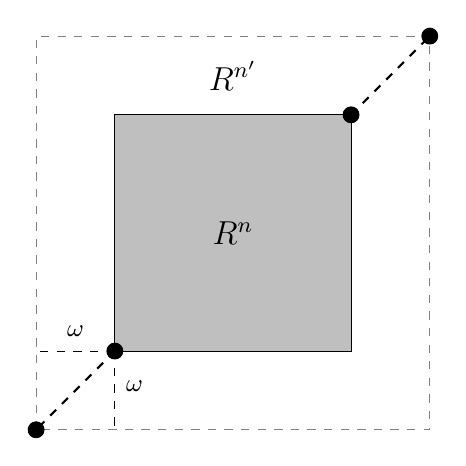
\begin{tikzpicture}[scale=.5]

%set up some coordinates 
%-----------------------
\coordinate (C1) at (0,0); % Outer top left
\coordinate (C2) at (10,10); % Outer bottom right
\coordinate (C3) at (2,2); % Inner top left
\coordinate (C4) at (8,8); % Inner bottom right

%draw figure contents
%--------------------

\draw [fill=lightgray] (C3) rectangle (C4); % Inner rectangle
\draw[dashed, color=gray] (C1) rectangle (C2); % Outer rectangle

\draw [fill] (C1) circle [radius=0.2]; % Outer top right
\draw [fill] (C2) circle [radius=0.2]; % Outer bottom left
\draw [fill] (C3) circle [radius=0.2]; % Inner top right
\draw [fill] (C4) circle [radius=0.2]; % Inner bottom left

\draw[thick,dashed] (C3) -- (C1); % Inner top right to outer top right
\draw[thick,dashed] (C4) -- (C2); % Inner bottom left to outer bottom left

\draw[dashed] (C3) -- (0,2);
\draw[dashed] (C3) -- (2,0);

\draw (5,5) node {\large $R^n$};
\draw (5,9) node {\large $R^{n'}$};

\draw (1,2.5) node {\small $\omega$}; % x1-w
\draw (2.5,1.1) node {\small $\omega$}; % y1-w

\end{tikzpicture}
\end{figure}

\end{frame}

\begin{frame}{Omregning fra punkt i billede til reelt punkt}







\end{frame}








